\documentclass[10pt,a4paper]{report}
\usepackage[utf8]{inputenc}
\usepackage[english]{babel}
\usepackage[T1]{fontenc}
\usepackage{amsmath}
\usepackage{amsfonts}
\usepackage{graphicx}
\usepackage{lmodern}
\usepackage{amssymb}
\usepackage{verbatim}
\usepackage{float}
\usepackage{amsthm}
\usepackage{hyperref}
\title{\LARGE{Algorithms for Computational Logic} \\ \vspace{0.5cm} \normalsize{Summary}}
\date{}

\begin{document}
\maketitle
\tableofcontents

\chapter{SAT and Modeling with SAT}
\section{Cardinality Constraints}
In order to handle cardinality constraints we have two options: encode the cardinality constraints to CNF and use a SAT solver, or use a pseudo boolean (PB) solver.
\subsection{AtMost1}
\begin{itemize}
\item $\sum_{j=1}^n x_j = 1$ can be encoded with $\left(\sum_{j=1}^n x_j \leq 1\right) \land \left(\sum_{j=1}^n x_j \geq 1\right)$
\item $\sum_{j=1}^n x_j \geq 1$ can be encoded with $(x_1 \lor x_2 \lor ... \lor x_n)$
\item $\sum_{j=1}^n x_j \leq 1$ can be encoded with:
\begin{itemize}
\item Pairwise encoding
\item Sequential counter encoding
\item Bitwise encoding
\end{itemize}
\end{itemize}
\subsubsection{Sequential Counter}
In order to realize this encoding, we need to add new variables $s_i$ for the fact "there is a 1 on some position $1..i$":
$$
s_i \text{ is true if } \sum_{j=1}^i x_j \geq 1
$$
Encoding $\sum_{j=1}^n x_j \leq 1$ with sequential counter:
\begin{align*}
&(\neg x_1 \lor s_1) \land\\
&(\neg x_i \lor s_i), i \in 2..n-1 \land\\
&(\neg s_{i-1} \lor s_i), i \in 2..n-1 \land\\
&(\neg x_i \lor \neg s_{i-1}), i \in 2..n
\end{align*}
If $x_j = 1$, then all $s_i$ variables are assigned and all other $x$ variables must take value 0. There are $\mathcal{O}(n)$ clauses and $\mathcal{O}(n)$ auxiliary variables.
\subsubsection{Bitwise Encoding}
In bitwise encoding, we represent the constraint $\sum_{j=1}^n x_j \leq 1$ by encoding the index of the potential true variable in binary. For this, we add new auxiliary variables:
$$
v_0, ... v_r-1;\; r=\lceil \log n \rceil (\text{with } n > 1)
$$
Each variable $x_j$ is assigned a unique binary number that represents its index. Then, for each variable $x_j$ with binary index representation $i$, we create clauses that enforce the condition: 
\begin{itemize}
    \item If $x_j = 1$, assignment to $v_i$ variables must encode $j - 1$, and all other $x$ variables must take value 0
    \item If all $x_j = 0$, any assignment to $v_i$ variables is consistent
\end{itemize}
For example, $x_1 + x_2 + x_3 \leq 1$:\\
\begin{minipage}{0.4\textwidth} 
    \centering
    \begin{table}[H]
        \begin{tabular}{ccc}
              & $j-1$ & $v_1v_0$ \\ \cline{1-3}
        $x_1$ & 0     & 00   \\
        $x_2$ & 1     & 01  \\
        $x_3$ & 2     & 10   
        \end{tabular}
    \end{table}
\end{minipage}
\begin{minipage}{0.55\textwidth} 
    \begin{align*}
        &(\neg x_1 \lor \neg v_1) \land (\neg x_1 \lor \neg v_0)\\
        &(\neg x_2 \lor \neg v_1) \land (\neg x_2 \lor v_0)\\
        &(\neg x_3 \lor v_1) \land (\neg x_3 \lor \neg v_0)\\
    \end{align*}
\end{minipage}
There are $\mathcal{O}(n\log n)$ clauses and $\mathcal{O}(\log n)$ auxiliary variables

\subsection{General Cardinality Constraints}
Constraints of the form $\sum_{j=1}^n x_j \leq k$ or $\sum_{j=1}^n x_j \geq k$ can be added with:
\begin{itemize}
    \item Sequential Counters
    \item BDDs
    \item Sorting Networks
    \item Cardinality Networks
    \item Totalizer
\end{itemize}
\subsubsection{Sequential Counter Encoding}
For each variable $x_i$, create k additional variables $s_{i,j}$ that are used as counters:
\begin{itemize}
    \item $s_{i,j} = 1$ if at least $j$ variables $\{x_1 ... x_i\}$ are assigned value 1
    \item $s_{i,j} = 0$ if at most $j - 1$ variables $\{x_1 ... x_i\}$ are assigned value 1
\end{itemize}
Encoding:
\begin{figure}[H]
    \centering
    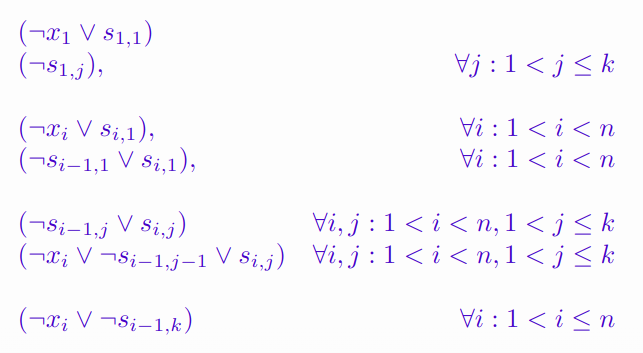
\includegraphics[scale=0.4]{1.png}
\end{figure}
\subsubsection{Totalizer Encoding}
In this encoding we count in unary how many of the $n$ variables $(x_1 ... x_n)$ are assigned to 1. It can be visualized as a tree:
\begin{itemize}
    \item Each node is ($name$ : $variable$ : $sum$)
    \item Root node has the output variables $(o_1 ... o_n)$ that count how many variables are assigned to 1
    \item Literals are at the leaves
    \item Each node counts in unary how many leaves are assigned to 1 in its subtree
    \item Example: if $b_2 = 1$, then at least 2 of the leaves $(x_3, x_4, x_5)$ are
    assigned to 1
\end{itemize}
\begin{figure}[H]
    \centering
    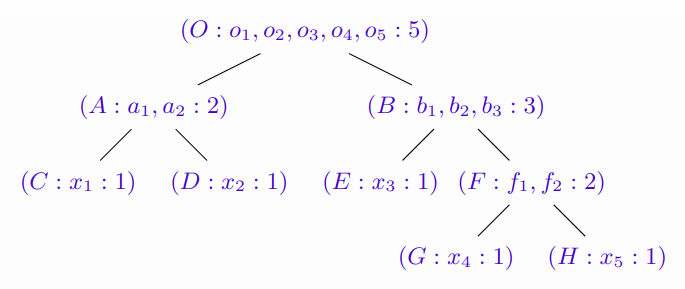
\includegraphics[scale=0.5]{2.png}
\end{figure}
To encode $x_1 + x_2 + x_3 + x_4 + x_5 \leq 3$ just set $o_4=0$ and $o_5=0$.\\
Encoding:
\begin{figure}[H]
    \centering
    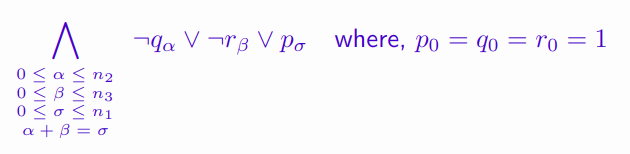
\includegraphics[scale=0.5]{3.png}
\end{figure}
There are $\mathcal{O}(n\log n)$ new variables and $\mathcal{O}(n^2)$ new clauses

\section{Pseudo-Boolean Constraints}
The general form of these constraints is $\sum_{j=1}^n a_jx_j \leq b$
\subsection{Encodings}
\subsubsection{BDD Encoding}
BDDs can be used to encode pseudo-boolean constraints. For example, to encode $3x_1 + 3x_2 + x_3 \leq 3$, we can construct the following BDD and extract its ITE-based circuit:
\begin{figure}[H]
    \centering
    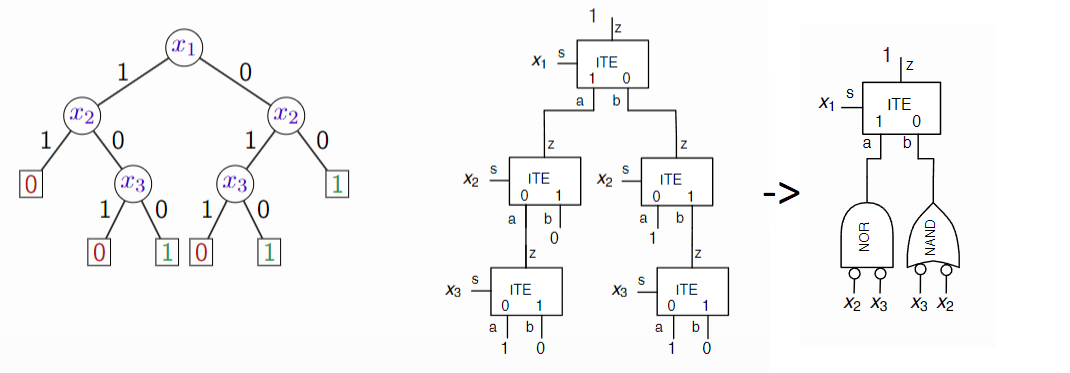
\includegraphics[scale=0.5]{18.png}
\end{figure}
\subsubsection{Sequential Weighted Counter Encoding}
Assuming the general form $\sum_{i=1}^n w_ix_i \leq k$, where the weights are all non-negative:
\begin{itemize}
    \item For each variable $x_i$, create $k$ additional variables $s_{i,j}$ that are used as counters
    \begin{itemize}
        \item $s_{i,j} = 1$ if the weighted sum of the first $i$ variables $\{x_1 . . . x_i\}$ is at least $j$
        \item $s_{i,j} = 0$ if the weighted sum of the first $i$ variables $\{x_1 . . . x_i\}$ is at most $j-1$
    \end{itemize}
\end{itemize}
Encoding:
\begin{figure}[H]
    \centering
    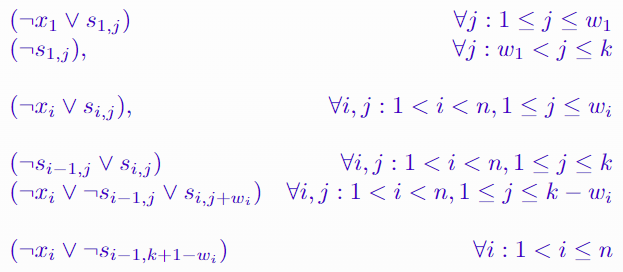
\includegraphics[scale=0.5]{19.png}
\end{figure}
\subsubsection{Generalized Totalizer Encoding}
The goal of GTE  is to account for the possible values of the left-hand side. It only considers the possible sums generated from the weights in the constraint. For example, in $2x_1 + 3x_2 + 3x_3 + 3x_4 \leq 5$ it is not possible for the weighted sum to have value 1, 4 or 7.
\begin{figure}[H]
    \centering
    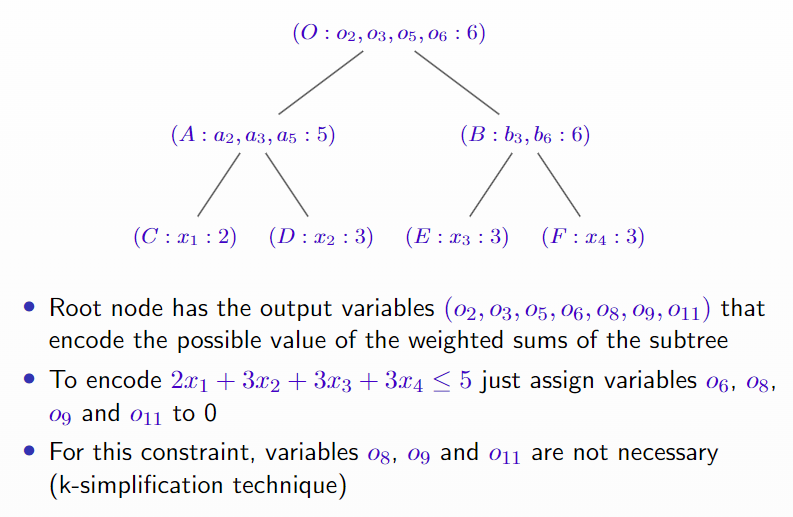
\includegraphics[scale=0.5]{20.png}
\end{figure}
\subsection{Pseudo-Boolean Optimization}
Suppose we must minimize $\sum_{j=1}^n c_jx_j$ subject to $\sum_{j=1}^n a_{ij}x_j \leq b_i \;\; \forall i \in \{1, ..., m\}, \forall j \in \{1, ..., n\}, x_j \in \{0, 1\}$. To translate this to MaxSAT we should:
\begin{itemize}
    \item Encode each pseudo-Boolean constraint into CNF. All clauses used in the encoding are hard
    \item For each term $c_jx_j$ in the objective function, add a soft clause $(\lnot x_j)$ with weight $c_j$
\end{itemize}
There are several ways of solving the optimization problem:
\begin{itemize}
    \item Translate into MaxSAT and use a Weighted MaxSAT algorithm
    \item Iterative Pseudo-Boolean solving
    \item Core-guided Pseudo-Boolean solving
    \item Branch-and-Bound Search
\end{itemize}
Given a PBO problem instance, where variables have an integer
domain, the Linear Programming Relaxation is the corresponding
linear program where the variable's integer constraints are relaxed
\begin{figure}[H]
    \centering
    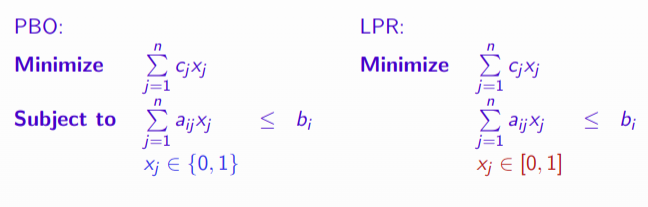
\includegraphics[scale=0.5]{21.png}
\end{figure}
\subsubsection{Linear Programming Relaxation}
LPR is relevant since if can be solved quickly and if he relaxed linear program returns an optimal solution where all variables have integer value, then the solution of the relaxed linear program is also the optimal solution of the PBO problem. If the solution of the relaxed linear program is not integer for some variable, it still provides a lower bound on the optimal value of the PBO optimal solution
\subsubsection{Branch-and-Bound Search}
In the branch and bound algorithm we search by recursively dividing into smaller subproblems. It continuously uses LPR to get lower bounds (in case of minimization) and get candidade solutions.
\begin{figure}[H]
    \centering
    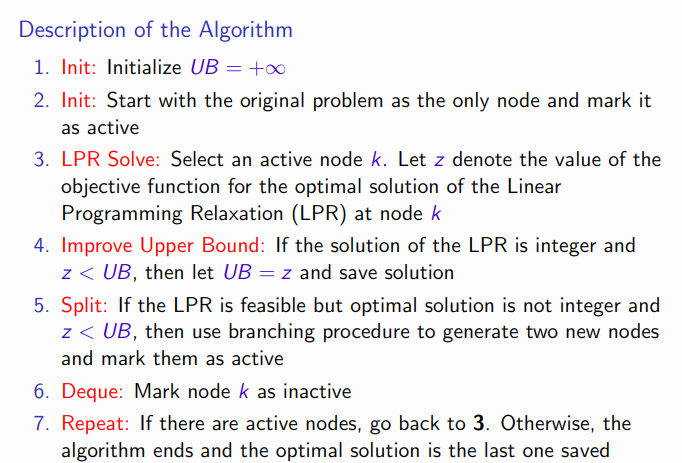
\includegraphics[scale=0.5]{22.png}
\end{figure}
\subsection{Cutting Planes}
Cutting planes are used to further prune the space. Can be used to combine two constraints:
\begin{figure}[H]
    \centering
    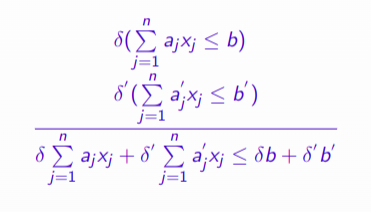
\includegraphics[scale=0.5]{23.png}
\end{figure}
For example:
\begin{figure}[H]
    \centering
    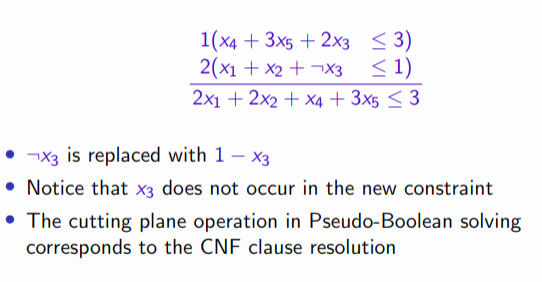
\includegraphics[scale=0.5]{24.png}
\end{figure}
Rounding can also be applied:
\begin{figure}[H]
    \centering
    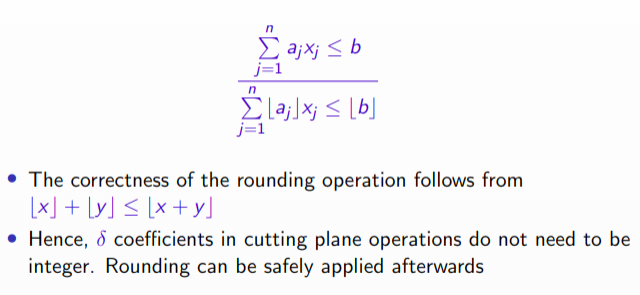
\includegraphics[scale=0.5]{25.png}
\end{figure}
For example:
\begin{figure}[H]
    \centering
    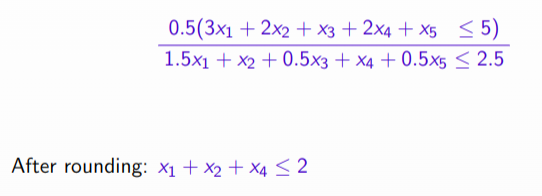
\includegraphics[scale=0.5]{26.png}
\end{figure}
And backtracking can also be applied:
\begin{figure}[H]
    \centering
    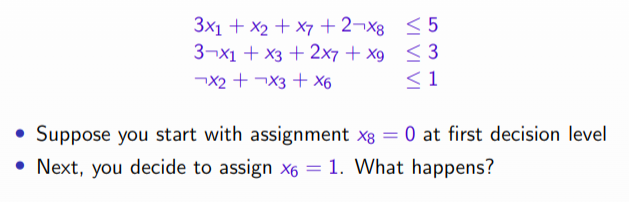
\includegraphics[scale=0.5]{27.png}
\end{figure}
\begin{figure}[H]
    \centering
    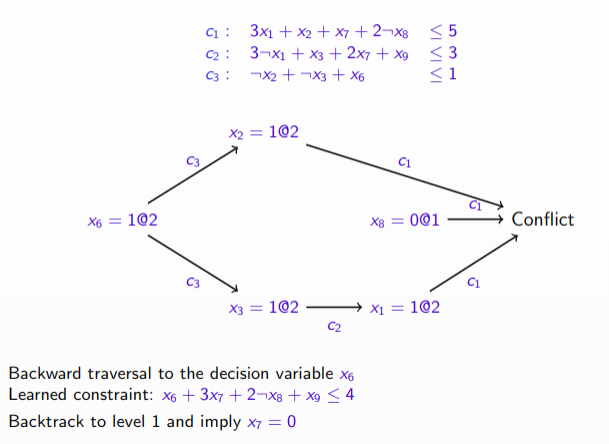
\includegraphics[scale=0.5]{28.png}
\end{figure}


\section{SAT Algorithms}
\subsection{DPLL Solvers}
\begin{figure}[H]
    \centering
    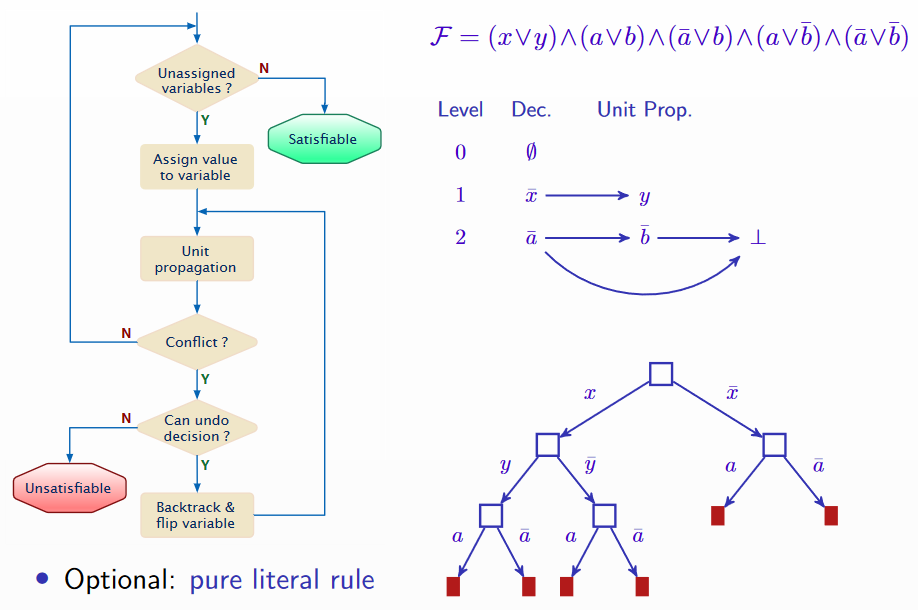
\includegraphics[scale=0.5]{4.png}
\end{figure}
\subsection{CDCL Solvers}
CDCL solvers extend DPLL solvers with clause learning and non-chronological backtracking, search restarts, lazy data structures, conflict-guided branching, etc.
\subsubsection{Clause Learning}
\begin{figure}[H]
    \centering
    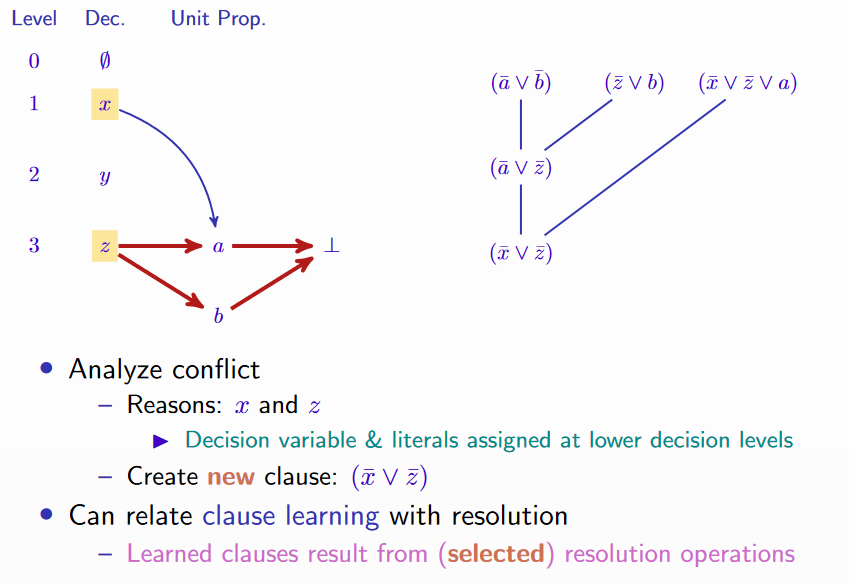
\includegraphics[scale=0.5]{5.png}
\end{figure}
And after backtracking:
\begin{figure}[H]
    \centering
    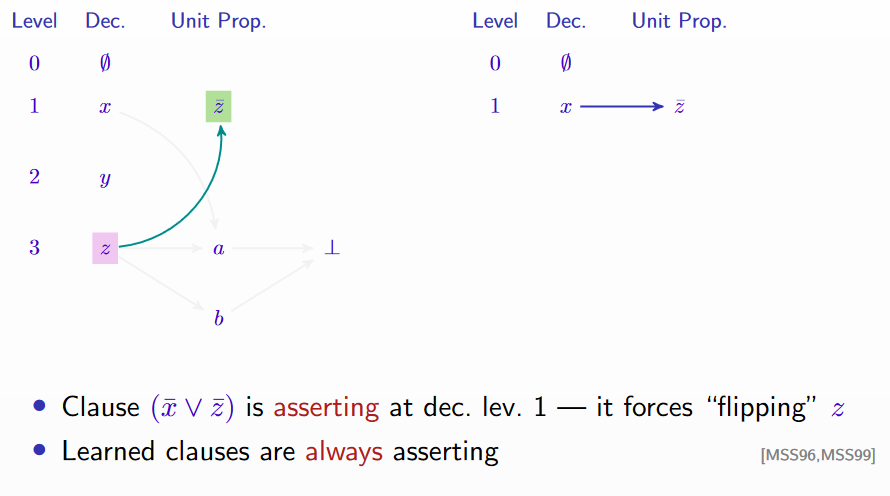
\includegraphics[scale=0.5]{6.png}
\end{figure}
\subsubsection{Unique Implication Points}
\begin{figure}[H]
    \centering
    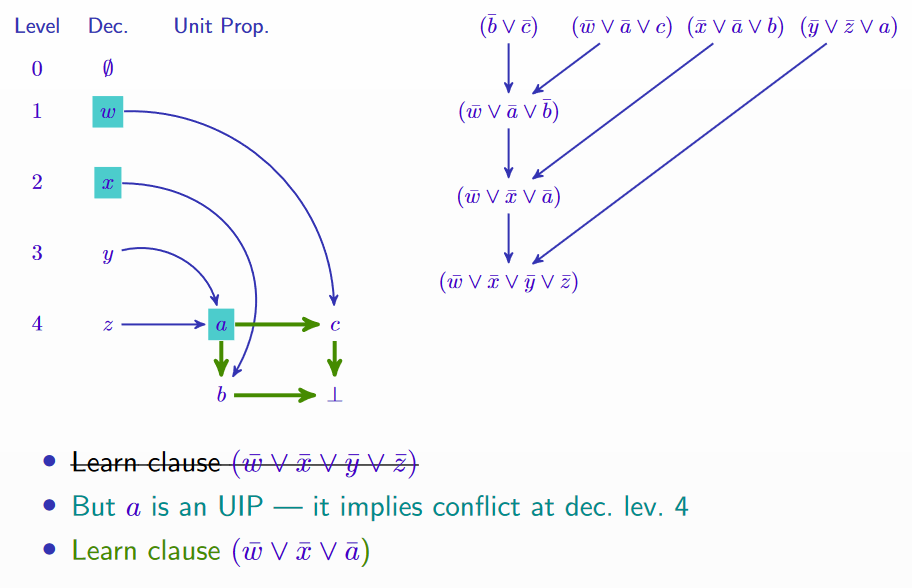
\includegraphics[scale=0.5]{7.png}
\end{figure}
\subsubsection{Clause Minimization}
\begin{figure}[H]
    \centering
    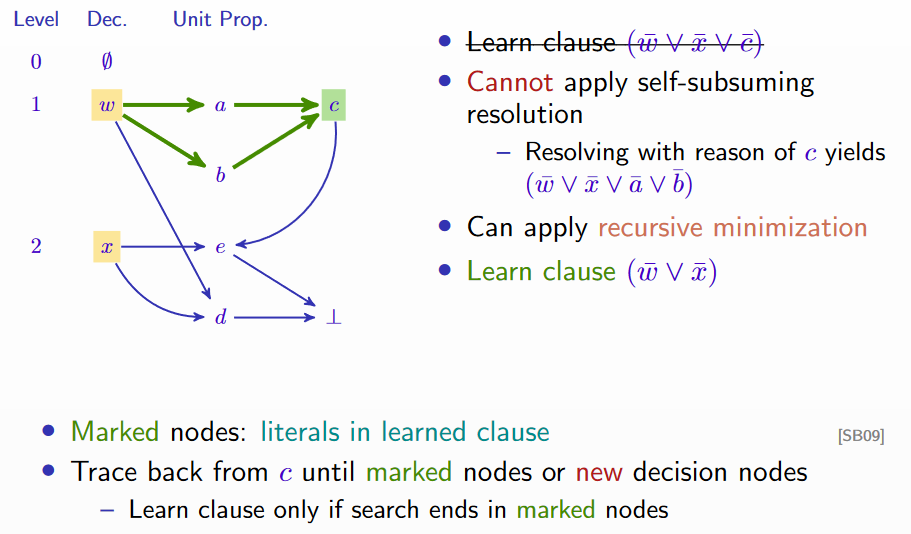
\includegraphics[scale=0.5]{8.png}
\end{figure}

\chapter{Optimization problems and SAT-Based Problem Solving}
A set of constraints is overconstrained if it is inconsistent. In a given an unsatisfiable formula, there may be several explanations for its unsatisfiability. The goal of MaxSAT is to find largest subset of clauses that is satisfiable.
\begin{figure}[H]
    \centering
    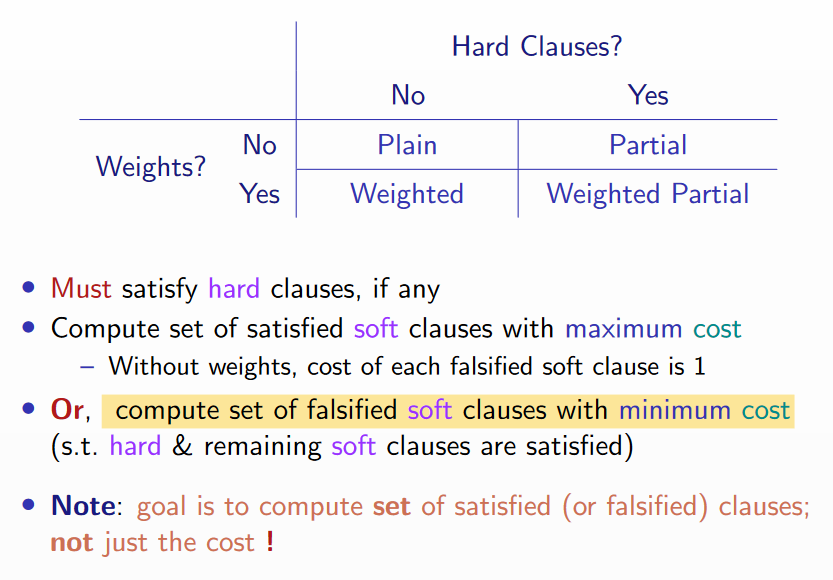
\includegraphics[scale=0.5]{9.png}
\end{figure}

\section{MaxSAT Algorithms}
\subsection{Fu and Malik}
\begin{figure}[H]
    \centering
    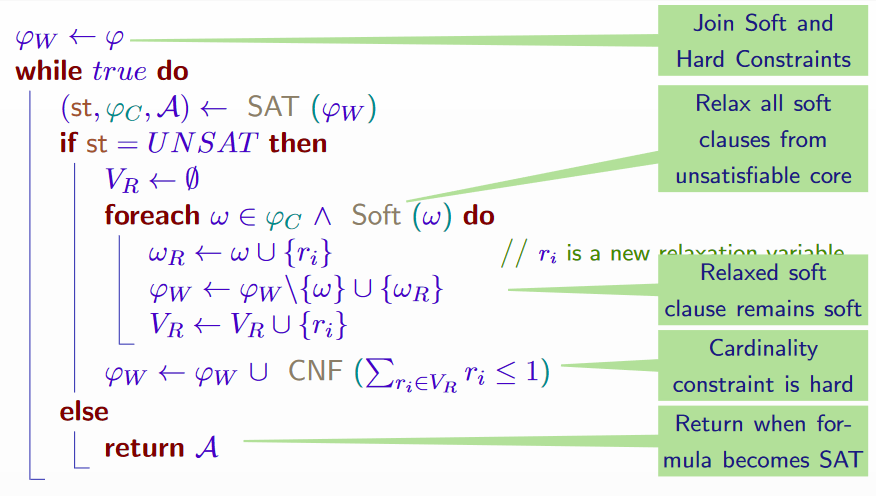
\includegraphics[scale=0.5]{10.png}
\end{figure}
\subsection{MSU3}
\begin{figure}[H]
    \centering
    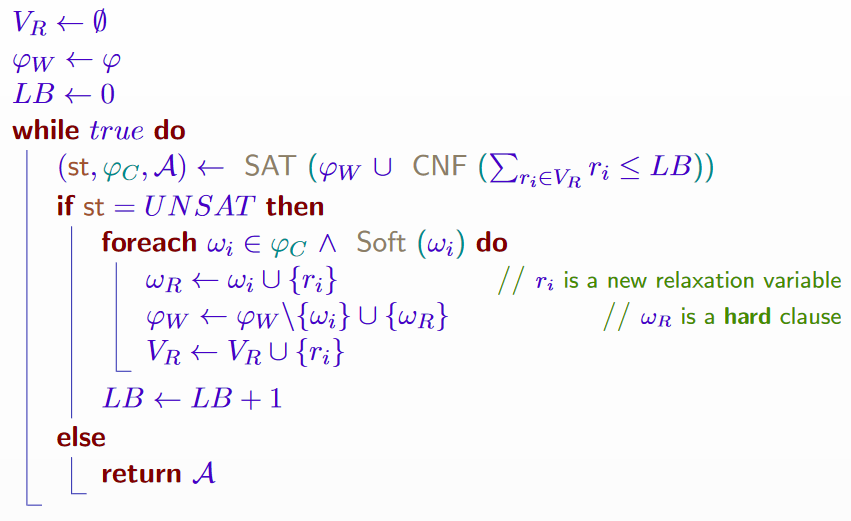
\includegraphics[scale=0.5]{11.png}
\end{figure}

\section{Minimal Unsatisfiable Subsets}
Given $\mathcal{F}$ unsatisfiable, $\mathcal{M} \subseteq \mathcal{F}$ is a MUS iff $\mathcal{M}$ is unsatisfiable and $\forall_{c \in \mathcal{M}}, \mathcal{M} \setminus \{c\}$ is satisfiable.
\subsection{Algorithms}
The following algorithms may be used to identify minimal unsatisfiable subsets.
\subsubsection{Deletion-Based}
\begin{figure}[H]
    \centering
    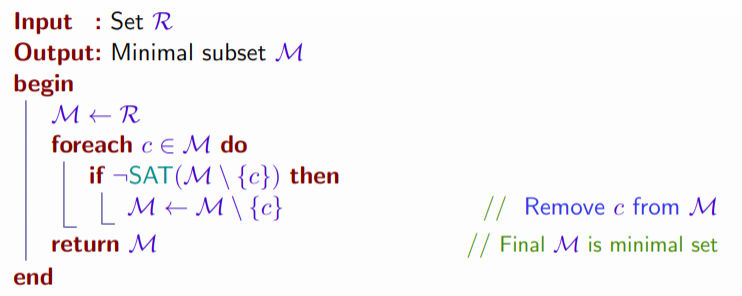
\includegraphics[scale=0.5]{12.png}
\end{figure}
\subsubsection{Insertion-Based}
\begin{figure}[H]
    \centering
    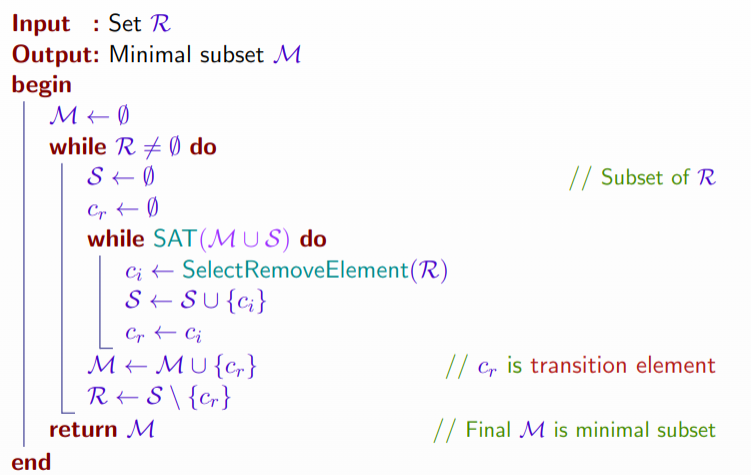
\includegraphics[scale=0.5]{13.png}
\end{figure}
\subsubsection{Dichotomic}
\begin{figure}[H]
    \centering
    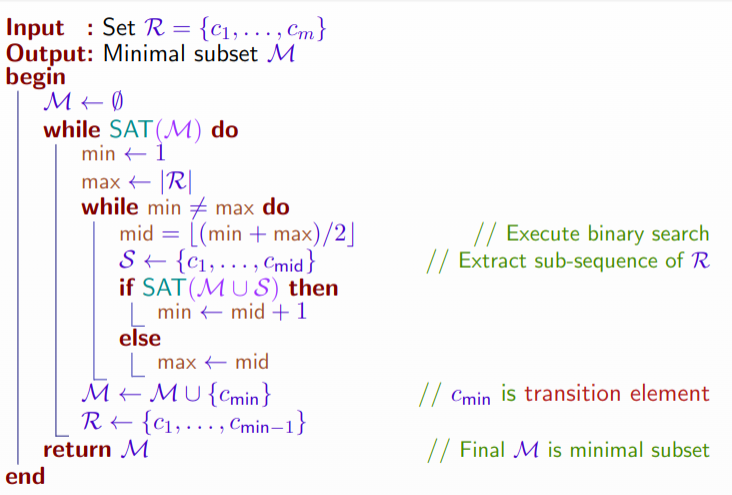
\includegraphics[scale=0.5]{14.png}
\end{figure}

\section{Minimal Correction Subsets}
$\mathcal{C} \subseteq \mathcal{F}$ is an MCS iff $\mathcal{F} \setminus \mathcal{C}$ is satisfiable and $\forall_{c \in \mathcal{C}}, \mathcal{F} \setminus (\mathcal{C} \setminus \{c\})$ is unsatisfiable.
\subsection{Algorithms}
The following algorithms may be used to identify minimal correction subsets.
\subsubsection{Basic Linear Search}
\begin{itemize}
    \item Let $\mathcal{S} \subseteq \mathcal{F}$, such that $\mathcal{S}\nvDash \bot$, initially $\mathcal{S} = \emptyset$
    \item Let $\mathcal{C} \subseteq \mathcal{F}$, such that $\forall_{c \in \mathcal{C}}, \mathcal{S} \cup \{c\} \vDash \bot $, initially $\mathcal{C} = \emptyset$
    \item At each iteration, analyze one clause of $c \in \mathcal{F} \setminus (\mathcal{S} \cup \mathcal{C})$:
    \begin{itemize}
        \item If $\mathcal{S} \cup \{c\} \vDash \bot$, then add $c$ to $\mathcal{C}$, i.e. $c$ is part of MCS
        \item If $\mathcal{S} \cup \{c\} \nvDash \bot$, then add $c$ to $\mathcal{C}$, i.e. $c$ is part of MCS
    \end{itemize}
\end{itemize}
There are $\mathcal{O}(m)$ calls to the oracle. An example:
\begin{figure}[H]
    \centering
    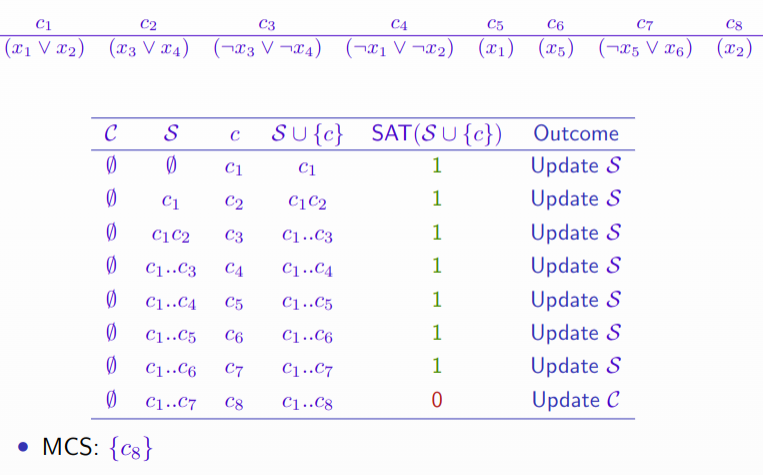
\includegraphics[scale=0.4]{15.png}
\end{figure}
\subsubsection{Clause D}
\begin{itemize}
    \item Pick an assignment and let $\mathcal{S} \subseteq \mathcal{F}$ be the satisfied clauses and $\mathcal{U} \subseteq \mathcal{F}$ be the falsified clauses, with $\mathcal{F} = \mathcal{S} \cup \mathcal{U}$
    \item Repeat:
    \begin{itemize}
        \item Create clause $D = \cup_{l \in c, c \in \mathcal{U}} l$
        \item If $\mathcal{S} \cup \{D\} \vDash \bot$, then $\mathcal{U}$ is MCS: Report MCS and terminate
        \item If $\mathcal{S} \cup \{D\} \nvDash \bot$, then add to $\mathcal{S}$ the satisfied clauses in $\mathcal{U}$, remove from $\mathcal{U}$ the satisfied clauses and loop
    \end{itemize}
\end{itemize}
There are $\mathcal{O}(m-r)$ calls to the oracle, where $r$ is the size of the smallest MCS. An example:
\begin{figure}[H]
    \centering
    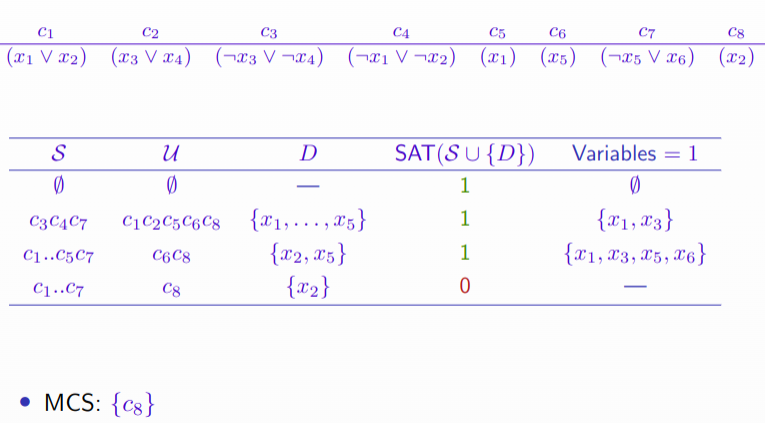
\includegraphics[scale=0.4]{16.png}
\end{figure}

\section{Duality Between MUSes and MCSes}
\begin{itemize}
    \item Let $\mathcal{S}$ be a finite set
    \item Let $\mathcal{F}$ be a set of subsets of $\mathcal{S}, \mathcal{F} \subseteq 2^\mathcal{S}$
    \item A hitting set $\mathcal{H} \subseteq \mathcal{S}$ is such that $\forall_{\mathcal{G} \in \mathcal{F}} \mathcal{H} \cap \mathcal{G} \neq \emptyset$
    \item $\mathcal{H}$ is (subset) minimal  if none of its subsets is a hitting set of $\mathcal{F}$
    \item $\mathcal{H}$ is cardinality minimal (or of minimum size) if there are no hitting sets of $\mathcal{F}$ with fewer elements
\end{itemize}
For example:
\begin{align*}
    &\mathcal{S} = \{1, 2, 3, 4, 5, 6, 7\}\\
    &\mathcal{F} = \{\{1, 2, 3\}, \{3, 4, 5\}, \{5, 6, 7\}\}\\
    &\mathcal{H}_1 = \{1, 2, 4, 6, 7\}\\
    &\mathcal{H}_1 = \{2, 4, 6\}\\
    &\mathcal{H}_1 = \{3, 7\}
\end{align*}
MUSes are minimal hitting sets of MCSes, and MCSes are minimal hitting sets of MUSes. En example:
\begin{figure}[H]
    \centering
    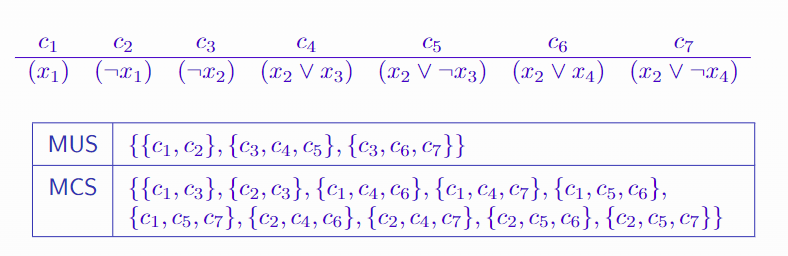
\includegraphics[scale=0.5]{17.png}
\end{figure}
\subsection{MHS Approach for Solving MaxSAT}
The MaxSAT solution is a smallest MCS, and any MCS is a hitting set of all MUSes. This duality can be used to solve MaxSAT:
\begin{enumerate}
    \item Let $\mathcal{K}$ be a set of unsatisfiable cores (or MUSes)
    \item Find a minimum hitting set $\mathcal{H}$ of the set $\mathcal{K}$ of already computed cores (or MUSes)
    \item Check satisfiability of $\mathcal{F} \setminus \mathcal{H}$
    \begin{itemize}
        \item If satisfiable, then $\mathcal{H}$ is a smallest MCS; terminate and return $\mathcal{H}$
        \item Otherwise, compute core (or MUS) and add it to $\mathcal{K}$
    \end{itemize}
    \item Loop from 2
\end{enumerate}
\subsection{Enumeration}
\subsubsection{MCSes}
Generate and block:
\begin{enumerate}
    \item Extract MCS $\mathcal{C}$
    \item Block $\mathcal{C}$, i.e. at least one clause in $\mathcal{C}$ must be satisfied
    \item Loop from 1
\end{enumerate}
\subsubsection{MUSes}
The process for enumerating MUSes is different since we cannot block them: preventing a clause from being added to the MUS is infeasible. The only solution is explicit set enumeration. Compute all MCSes and then all MUSes:
\begin{itemize}
    \item Compute all MCSes using MCS enumerator
    \item Compute all minimal hitting sets of the MCSes
\end{itemize}

\chapter{Satisfiability Modulo Theories}
\chapter{Answer Set Programming}
\end{document}
